\documentclass[ngerman,compress]{beamer}

\mode<presentation>
{
  \useoutertheme[footline=titleinstituteauthor]{c4}
  \useinnertheme{circles}
  \usecolortheme{c4}
  %\setbeamercovered{transparent}
  \setbeamercovered{highly dynamic}
}

\usepackage{babel}
\usepackage[utf8]{luainputenc}
\usepackage{fontspec}
\usepackage{listings}
\usepackage{color}
\usepackage{mathtools}

% Multimedia
%\usepackage{multimedia}

% sets the listings style
\definecolor{sh_comment}{rgb}{0.12, 0.38, 0.18 } %adjusted, in Eclipse: {0.25, 0.42, 0.30 } = #3F6A4D
\definecolor{sh_keyword}{rgb}{0.3, 0.3, 0.875}  % #5F1441
\definecolor{sh_string}{rgb}{0.875, 0.85, 0.11} % #101AF9

\lstset{basicstyle=\tiny\ttfamily,
	showspaces=false,
	showtabs=false,
	showstringspaces=false,
	columns=fullflexible,
	stringstyle=\color{sh_string},
	keywordstyle=\color{sh_keyword}\bfseries,
	commentstyle=\color{sh_comment}\itshape
	}

\title[STM32 - GPIO und Timer - u23 2013]
{\textbf{STM32 - GPIO und Timer}\\u23 2013}

\author[andy <andy@koeln.ccc.de>]
{andy, florob, gordin, ike, meise, tobix, zakx}

\institute[Chaos Computer Club Cologne]
{
Chaos Computer Club Cologne e.V.\\
http://koeln.ccc.de \\
}

\date{Cologne\\2013-10-28}

\pgfdeclareimage[height=1cm]{barcode}{./c4-logo}
\logo{\pgfuseimage{barcode}}


% Folgendes sollte gelC6scht werden, wenn man nicht am Anfang jedes
% Unterabschnitts die Gliederung nochmal sehen möchte.
%\AtBeginSection[]
%{
%  \begin{frame}<beamer>
%    \frametitle{Gliederung}
%    \tableofcontents[currentsection,currentsubsection]
%  \end{frame}
%}

% Falls Aufzählungen immer schrittweise gezeigt werden sollen, kann
% folgendes Kommando benutzt werden:
%\beamerdefaultoverlayspecification{<+->}


\begin{document}

\begin{frame}
  \titlepage
\end{frame}

\AtBeginSubsection

\begin{frame}
  \tableofcontents
  % Die Option [pausesections] könnte nützlich sein.
\end{frame}


\section{GPIO}

\subsection{GPIOs}

\begin{frame}
	\frametitle{GPIO}
	\begin{itemize}
		\item GPIO = \textbf{G}eneral \textbf{P}urpose \textbf{I}nput/\textbf{O}utput
		\item = durch Software wackelnde Pins am Mikrocontroller
		\item Kennen zwei Modi: Input und Output
		\item Standardkonfiguration eines Pins = GPIO Input
		\item STM32F4 hat GPIOA bis GPIOI mit je 16 Pins (ne Menge!)
		\item Als Vergleich Atmega32: GPIOA bis GPIOD mit je 8 Pins
	\end{itemize}
\end{frame}

\begin{frame} [fragile]
	\frametitle{Konfiguration}
	Der Kram muss konfiguriert werden:
	\begin{lstlisting} [language=C]
	GPIO_InitTypeDef  GPIO_InitStructure;

	/* Enable the GPIO_LED Clock */
	RCC_AHB1PeriphClockCmd(RCC_AHB1Periph_GPIOD, ENABLE);

	/* Configure the GPIO_LED pins */
	GPIO_InitStructure.GPIO_Pin = GPIO_Pin_12 | GPIO_Pin_13 | GPIO_Pin_14 | GPIO_Pin_15;
	GPIO_InitStructure.GPIO_Mode = GPIO_Mode_OUT;
	GPIO_InitStructure.GPIO_OType = GPIO_OType_PP;
	GPIO_InitStructure.GPIO_PuPd = GPIO_PuPd_UP;
	GPIO_InitStructure.GPIO_Speed = GPIO_Speed_50MHz;
	GPIO_Init(GPIOD, &GPIO_InitStructure);
	\end{lstlisting}
\end{frame}

\begin{frame} [fragile]
	\frametitle{Der Reihe nach (1)}
	Clock einschalten, damit der GPIO-Kern irgendwas tut:
	\begin{lstlisting} [language=C, basicstyle=\small]
	/* Enable the GPIO Clock */
	RCC_AHB1PeriphClockCmd(RCC_AHB1Periph_GPIOD, ENABLE);
	\end{lstlisting}
\end{frame}

\begin{frame} [fragile]
	\frametitle{Der Reihe nach (2)}
	Wir konfigurieren hier Pins 12 bis 15 ...
	\begin{lstlisting} [language=C, basicstyle=\small, breaklines=true]
	GPIO_InitStructure.GPIO_Pin = GPIO_Pin_12 | GPIO_Pin_13 | GPIO_Pin_14 | GPIO_Pin_15;
	\end{lstlisting}
	\pause
	... als Ausgänge ...
	\begin{lstlisting} [language=C, basicstyle=\small]
	GPIO_InitStructure.GPIO_Mode = GPIO_Mode_OUT;
	\end{lstlisting}
	\pause
	... im Modus Push/Pull ...
	\begin{lstlisting} [language=C, basicstyle=\small]
	GPIO_InitStructure.GPIO_OType = GPIO_OType_PP;
	\end{lstlisting}
\end{frame}

\begin{frame} [fragile]
	\frametitle{Der Reihe nach (3)}
	... mit aktiviertem Pullup (eigentlich sinnfrei bei Push-Pull-Ausgängen) ...
	\begin{lstlisting} [language=C, basicstyle=\small]
	GPIO_InitStructure.GPIO_PuPd = GPIO_PuPd_UP;
	\end{lstlisting}
	\pause
	... und max. 50 MHz Geschwindigkeit.
	\begin{lstlisting} [language=C, basicstyle=\small]
	GPIO_InitStructure.GPIO_Speed = GPIO_Speed_50MHz;
	\end{lstlisting}
	\pause
	BÄM!
	\begin{lstlisting} [language=C, basicstyle=\small]
	GPIO_Init(GPIOD, &GPIO_InitStructure);
	\end{lstlisting}
\end{frame}

\begin{frame} [fragile]
	\frametitle{Pins nutzen}
	So setzt man Pins:
	\begin{lstlisting} [language=C, basicstyle=\small]
	GPIO_SetBits(GPIOD, GPIO_Pin_12 | GPIO_Pin_15);
	\end{lstlisting}
	\pause
	So löscht man Pins:
	\begin{lstlisting} [language=C, basicstyle=\small]
	GPIO_ResetBits(GPIOD, GPIO_Pin_13 | GPIO_Pin_14);
	\end{lstlisting}
	\pause
	So liest man Pins:
	\begin{lstlisting} [language=C, basicstyle=\small]
	if(GPIO_ReadInputDataBit(GPIOA, GPIO_Pin_0) == Bit_SET)
	{
		...
	}
	\end{lstlisting}
	Noch mehr, lest das mal selbst nach: \emph{stm32f4xx\_gpio.h}
\end{frame}


\begin{frame}
	\frametitle{Pullup/down Widerstände}
	Annahme: Wir klemmen einen Schalter an einen Input an.
	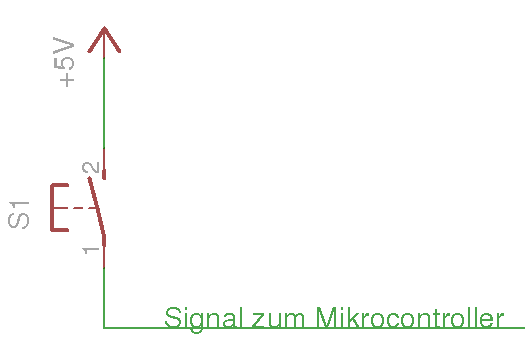
\includegraphics[height=1.5in]{keinpullupdown.png}
	\begin{enumerate}
		\item Welchen Pegel hat der Mikrocontrollerpin, wenn der Schalter geschlossen ist?
		\item Welchen Pegel hat der Mikrocontrollerpin, wenn der Schalter offen ist?
	\end{enumerate}
\end{frame}

\begin{frame}
	\frametitle{Pullup-Widerstand}
	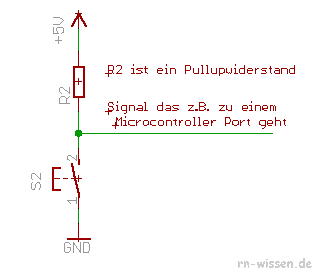
\includegraphics[height=1.5in]{Pullup.png}
	\begin{enumerate}
		\item Welchen Pegel hat der Mikrocontrollerpin, wenn der Schalter geschlossen ist?
		\item Welchen Pegel hat der Mikrocontrollerpin, wenn der Schalter offen ist?
	\end{enumerate}
\end{frame}

\begin{frame}
	\frametitle{Pulldown-Widerstand}
	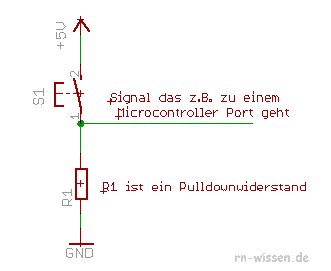
\includegraphics[height=1.5in]{Pulldown.png}
	\begin{enumerate}
		\item Welchen Pegel hat der Mikrocontrollerpin, wenn der Schalter geschlossen ist?
		\item Welchen Pegel hat der Mikrocontrollerpin, wenn der Schalter offen ist?
	\end{enumerate}
\end{frame}

\begin{frame}
	\frametitle{Pinmodi}
	\emph{GPIO\_Mode} ist ziemlich selbsterklärend:
	\begin{itemize}
		\item \emph{GPIO\_Mode\_IN} -- Input
		\item \emph{GPIO\_Mode\_OUT} -- Output
		\item \emph{GPIO\_Mode\_AF} -- Auxiliary Function
		\item \emph{GPIO\_Mode\_AN} -- Analog Input
	\end{itemize}
\end{frame}

\begin{frame}
	\frametitle{Pinmodi}
	\emph{GPIO\_OType} (O = Output) kennt nur zwei Modi:
	\begin{itemize}
		\item \emph{GPIO\_OType\_PP} -- Push/Pull = hartes ziehen oder drücken auf 0V oder 3,3V
		\item \emph{GPIO\_OType\_OD} -- OpenDrain = hartes ziehen auf 0V oder hochohmig (mit Pullup dann plötzlich high)
	\end{itemize}
\end{frame}

\begin{frame}
	\frametitle{Pinmodi}
	\emph{GPIO\_PuPd} kümmert sich um die Pullups/Downs:
	\begin{itemize}
		\item \emph{GPIO\_PuPd\_NOPULL} -- Kein Pullup/down
		\item \emph{GPIO\_PuPd\_UP} -- Pullup an
		\item \emph{GPIO\_PuPd\_DOWN} -- Pulldown an
	\end{itemize}
\end{frame}


\subsection{Interrupts durch GPIOs}

\begin{frame}
	\frametitle{GPIO Interrupts}
	Anstatt die ganze Zeit die Pins abzufragen, ob da was passiert ist, können sie auch Interrupts werfen. Sample dazu ist \emph{04\_gpiointerrupt}.
\end{frame}

\begin{frame} [fragile]
	\frametitle{GPIO Interrupts}
	Pin konfigurieren wie sonst auch. PA0 ist der User-Button, auf der Platine ist ein Pullup-Widerstand. Bonuspunkte für Leute die ihn mir im Schaltplan raussuchen und mir sagen wie er heisst und wie groß er ist.
	\begin{lstlisting} [language=C]
	//Clock einschalten
	RCC_AHB1PeriphClockCmd(RCC_AHB1Periph_GPIOA, ENABLE);

	// Pinmodus konfigurieren
	GPIO_Init(GPIOA, &(GPIO_InitTypeDef){
		.GPIO_Speed = GPIO_Speed_50MHz,
		.GPIO_Mode = GPIO_Mode_IN,
		.GPIO_OType = GPIO_OType_PP,
		.GPIO_PuPd = GPIO_PuPd_NOPULL,	//no internal pullup or pulldown, is present on PCB
		.GPIO_Pin = GPIO_Pin_0
	});
	\end{lstlisting}
\end{frame}

\begin{frame} [fragile]
	\frametitle{GPIO Interrupts}
	GPIO Interrupts werden durch den EXTI-Kern behandelt. Konfigurieren...
	\begin{lstlisting} [language=C]
	EXTI_Init(&(EXTI_InitTypeDef){
		.EXTI_Line = EXTI_Line0,
		.EXTI_Mode = EXTI_Mode_Interrupt,
		.EXTI_Trigger = EXTI_Trigger_Rising,
		.EXTI_LineCmd = ENABLE
	});
	\end{lstlisting}
	Was geht da? Ich bin faul findet das zur Abwechslung mal selbst raus ;) \emph{STM32 Reference Manual Page 199ff}
\end{frame}

\begin{frame} [fragile]
	\frametitle{GPIO Interrupts}
	Nur soviel:
	\begin{itemize}
		\item Es gibt 16 Leitungen im Chip: EXTI0 bis EXTI15
		\item An EXTI0 hängen: PA0, PB0, PC0, PD0, ..., PI0
		\item An EXTI1 hängen: PA1, PB1, PC1, PD1, ..., PI1
		\item ... klar, oder?
		\item Wir haben hier aber EXTI0 konfiguriert. Wie kriegen wir jetzt also PA0 and EXTI0?
	\end{itemize}
	\pause
	So:
	\begin{lstlisting} [language=C, basicstyle=\small]
	SYSCFG_EXTILineConfig(EXTI_PortSourceGPIOA, EXTI_PinSource0);
	\end{lstlisting}
\end{frame}

\begin{frame} [fragile]
	\frametitle{GPIO Interrupts}
	Als letztes müssen wir den Interrupt im Interrupt-Controller noch einschalten:
	\begin{lstlisting} [language=C, basicstyle=\small]
    NVIC_Init(&(NVIC_InitTypeDef){
        .NVIC_IRQChannel = EXTI0_IRQn,
        .NVIC_IRQChannelPreemptionPriority = 0x00,
        .NVIC_IRQChannelSubPriority = 0x00,
        .NVIC_IRQChannelCmd = ENABLE
    });
	\end{lstlisting}
\end{frame}

\begin{frame} [fragile]
	\frametitle{GPIO Interrupts}
	Und so sieht die Interruptroutine aus:
	\begin{lstlisting} [language=C, basicstyle=\small, breaklines=true]
void EXTI0_IRQHandler()
{
    //huh? You talking to me?
    if(EXTI_GetITStatus(EXTI_Line0) != RESET)
    {
        GPIO_ToggleBits(GPIOD, GPIO_Pin_12 | GPIO_Pin_13 | GPIO_Pin_14 | GPIO_Pin_15);

        //Clear the interrupt bit and tell the controller we handled the interrupt
        EXTI_ClearITPendingBit(EXTI_Line0);
    }
}
	\end{lstlisting}
\end{frame}

\begin{frame} [fragile]
	\frametitle{GPIO Interrupts}
	War viel? Keine Sorge, guckt ins Example 01 bis 04. Da steht alles kommentiert und zusammen in jeweils einem File.
\end{frame}


\section{Timer}

\subsection{Timer}

\begin{frame}
	\frametitle{Timer}
	\begin{itemize}
		\item Timer sind vom Konzept her relativ einfach, aber durch die vielfältigen Anwendungsgebiete doch relativ komplexe Biester
		\item Deswegen werden wir hier das Thema nur kurz anschneiden (wie leider fast alles -\_-)
		\item Ich beherrsche auch nicht alle Modi auswendig, mit Grundverständnis und etwas Googlen + Datasheets kommt man aber ganz gut hin
		\item Timer sind simpel: Sie haben ein x Bit breites Register und bei jedem Auftreten eines Clockimpulses wird das register inkrementiert
		\item Kühles Howto zum nachlesen: \url{http://visualgdb.com/tutorials/arm/stm32/timers/}
	\end{itemize}
\end{frame}

\begin{frame}
	\frametitle{Timer}
	Annahme: 16 Bit Timer, 40 MHz Clock, wie lange tickt das Ding, bis es überläuft?
	\begin{itemize}
		\item $2^{16} = 65536$, Wertebereich des Timers als 0 bis 65535
		\item $40MHz = 40*{10}^{6}$ Ticks pro Sekunde = 40 000 000 Hz
		\item Der Timer inkrementiert also 40000000 pro Sekunde
		\item Damit läuft der Timer als $40000000MHz/65536 = 610,3515625$ pro Sekunde über
		\item Somit ist $1s/610,3515625 = 0,0016384s = 1,6384ms$
		\pause
		\item \textbf{Würde man also einen 16 Bit Timer mit 40MHz von 0 an laufen lassen, hat man einen Überlauf alle 1,6384ms}
		\pause
		\item Rechnet mal, wie lange ein 32 Bit Timer bei 100 MHz braucht, bis der überläuft!
	\end{itemize}
\end{frame}

\begin{frame}
	\frametitle{Timer}
	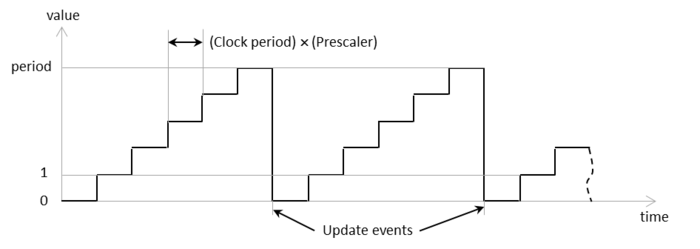
\includegraphics[height=1.7in]{01-timer.png} \\
	\footnotesize{Quelle: \url{http://visualgdb.com/tutorials/arm/stm32/timers/}}
\end{frame}

\begin{frame}
	\frametitle{Timer}
	Allgemeine Formeln
	\begin{itemize}
		\item $tickDauer = \frac{1}{timerFrequenz}$
		\item $zeitBis"Uberlauf = z"ahlSchritte * tickDauer$
	\end{itemize}
	Die Dinger sind so einfach, dass man sich die mit etwas Übung auch schnell selbst herleiten kann.
\end{frame}

\begin{frame}
	\frametitle{STM32 Timer}
	Welche Timer haben wir denn und wie schnell ticken die wirklich?
	\begin{itemize}
		\item Dieses clocking Excelsheet in \emph{docs/} verrät euch das
		\item TIM 1 und 8: 16 Bit
		\item TIM 2 bis 5: 16 Bit und 32 Bit
		\item TIM 9 bis 14: 16 Bit
		\item TIM 6 und 7: 16 Bit
		\item Verschiedene Timer haben verschiedene Features
		\item Wie immer alles im Datasheet
	\end{itemize}
\end{frame}

\begin{frame} [fragile]
	\frametitle{Timer konfigurieren}
	Wir konfigurieren mal einen Timer im sogenannten TimeBase Modus (geklaut aus \emph{05\_ledpwm}).
	\begin{lstlisting} [language=C]
//Enable Timer 4 clock
RCC_APB1PeriphClockCmd(RCC_APB1Periph_TIM4, ENABLE);

//We want the timer to tick with a frequency of 1MHz, calculate a prescaler
uint32_t PrescalerValue = (uint16_t) ((SystemCoreClock / 2) / 1000000) - 1;

//20 kHz PWM period (i.e. 50uS period)
uint32_t period = 1000000 / 20000;

//Configure the timer
TIM_TimeBaseInit(TIM4, &(TIM_TimeBaseInitTypeDef){
	.TIM_Period = period - 1,
	.TIM_Prescaler = PrescalerValue,
	.TIM_ClockDivision = 0,
	.TIM_CounterMode = TIM_CounterMode_Up,
});
	\end{lstlisting}
	Das Ding tickt einfach nur mit der angegebenen Frequenz vor sich hin. Mehr passiert da nicht.
\end{frame}

\begin{frame} [fragile]
	\frametitle{Timer konfigurieren}
Als letztes noch den Timer starten:
	\begin{lstlisting} [language=C, basicstyle=\small]
TIM_Cmd(TIM4, ENABLE);
	\end{lstlisting}
	Tick, tack... \\
\pause
Aktuellen Tickwert holen:
\begin{lstlisting} [language=C, basicstyle=\small]
TIM_GetCounter(TIM4);
	\end{lstlisting}
\end{frame}

\subsection{PWM}

\begin{frame}
	\frametitle{PWM}
	\begin{itemize}
		\item Jetzt, wo wir wissen, wie Timer generell funktionieren, lassen wir mal LEDs flackern
		\item Helligkeit von LEDs wird über PWM (= Pulse Width Modulation = Pulsweitenmodulation) ermöglicht
		\item Zu gut Deutsch: LED ist X\% der Gesamtzeit an und 100\%-X\% der Gesamtzeit aus
	\end{itemize}
\end{frame}

\begin{frame}
	\frametitle{PWM}
	\begin{itemize}
		\item Fürs messen von Zeiten nehmen wir immer Timer auf einem Mikrocontroller
		\item Wir machen die LED an, fangen bei 0 an zu Zählen und warten etwas
		\item Wenn der Timer einen gewissen Wert erreicht hat (= gewisse Zeit verstrichen ist), machen wir die LED wieder aus ...
		\item ... und warten, bis der Timer überläuft
		\item Wenn man das schnell genug macht, sieht man das als Mensch durch die Trägheit der Augen nichtmal
		\item Repeat...
		\pause
		\item Easy, oder?
	\end{itemize}
\end{frame}

\begin{frame}
	\frametitle{PWM}
	Rechenbeispiel:
	\begin{itemize}
		\item Eine Timerperiode ist 50µS lang
		\item Angenommen der Timer zählt innerhalb dieser 50µS immer bis 50 und wird dann wieder auf 0 zurückgesetzt ...
		\item ... und wir setzen den OutputCompare auf 25, ist 50\% der Zeit die LED an, sonst aus
		\item Bei 10 wären das 5µS an und den die Restlichen 45µS aus
	\end{itemize}
\end{frame}

\begin{frame}[fragile]
	\frametitle{Output Compare Config}
	Ich kopier mal wieder Code (\emph{05\_ledpwm}):
	\begin{lstlisting} [language=C, breaklines=true]
//PD12 auf Alternate Function legen (Achtung! Bei GPIO Config auch AF als Mode angeben!)
GPIO_PinAFConfig(GPIOD, GPIO_PinSource12, GPIO_AF_TIM4);

//Timer konfigurieren, so das er passend tickt
<...>

TIM_OCInitTypeDef TIM_OCInitStructure;
TIM_OCInitStructure.TIM_OCMode = TIM_OCMode_PWM1;
TIM_OCInitStructure.TIM_OutputState = TIM_OutputState_Enable;
TIM_OCInitStructure.TIM_Pulse = 0;
TIM_OCInitStructure.TIM_OCPolarity = TIM_OCPolarity_High;

// PWM1 Mode configuration: Channel1 (GPIOD Pin 12)
TIM_OC1Init(TIM4, &TIM_OCInitStructure);
TIM_OC1PreloadConfig(TIM4, TIM_OCPreload_Enable);

// Comparewert setzen
TIM_SetCompare1(TIM4, 10);
	\end{lstlisting}
\end{frame}




\section{Aufgaben}
\subsection{Aufgaben}
\begin{frame}
	\frametitle{GPIO-Aufgaben}
	\begin{enumerate}
		\item Versucht mal selbst die LEDs zum Blinken zu bringen (also selbst Pinmodi konfigurieren etc.)
		\item Versucht mal den Input für den Userbutton richtig zu konfigurieren und Dinge damit zu tun
		\item Probiert auch mal die Interrupts aus
		\item Was fällt euch auf, wenn ihr den Taster drückt? Wie oft wird eure programmierte Aktion pro Druck ausgelöst?
		\item Behebt das festgestellte Problem (entprellen)! Wie ist mir egal.
	\end{enumerate}
\end{frame}

\begin{frame}
	\frametitle{Timer-Aufgaben}
	\begin{enumerate}
		\item Konfiguriert mal einen Timer im TimeBase-Mode und lasst ihn mit einer von euch festgelegten Frequenz ticken (also ohne Output Compare oder son Kram, nur der Timer)
		\item Wenn das geht, könnt ihr in einer Schleife regelmäßig den Wert auslesen und ab einem Schwellwert ne LED an- und ausschalten -> Blinkerei! (siehe auch: \url{http://visualgdb.com/tutorials/arm/stm32/timers/})
		\item Spielt mal mit den Comparewerten in dem LED-PWM example und guckt was sich ändert. Ich komm dann mal mit nem Logicanalyzer rum und zeig auch live wie das aussieht.
	\end{enumerate}
\end{frame}

\begin{frame}
	\frametitle{Timer-Aufgaben}
	\begin{enumerate}
		\setcounter{enumi}{3}
		\item Wenn es euch interessiert, stellt den Timer mal so ein, dass er alle x Millisekunden überläuft und probiert mal in einem zweiten Schritt einen Interrupt bei einem Timer-Overflow zu erzeugen (Hints: \emph{TIM\_ITConfig()}, \emph{TIMx\_IRQHandler()}, \emph{TIM\_ClearITPendingBit()}, \emph{TIM\_GetITStatus()}). Damit könnt ihr jetzt relativ genau Zeit messen und wisst, wie die Delay()-Funktion funktioniert
	\end{enumerate}
\end{frame}

\begin{frame}
	\frametitle{Sonstiges}
	\begin{itemize}
		\item Letztes mal wollte jemand wissen, was das EVENTOUT das bei den meisten Pins als auxiliary function zu sehen war bedeutet. Hier stehts: \url{http://electronics.stackexchange.com/questions/28740/what-is-the-stm32-event-eventout}
		\item Spielt mal damit, wenn ihr Lust habt, das hört sich lustig an!
	\end{itemize}
\end{frame}

\end{document}
